\documentclass[UTF8]{ctexart}
\usepackage{subfigure}
\usepackage{caption}
\usepackage{amsmath,bm}
\usepackage{amssymb}
\usepackage{pifont}
\usepackage{geometry}
\usepackage{graphicx}
\usepackage{gensymb}
\usepackage{wrapfig}
\usepackage{titlesec}
\usepackage{float}
\usepackage{diagbox}
\usepackage{fancyhdr}
\usepackage{color}
\usepackage{bm}
\usepackage{siunitx}
\pagestyle{plain}
\geometry{a4paper,scale=0.8}
\CTEXsetup[format+={\raggedright}]{section} 
\title{量统2016-2017郭永期末}
\author{Deschain}
\titlespacing*{\section}
{0pt}{0pt}{0pt}
\titlespacing*{\subsection}
{0pt}{0pt}{0pt}
\titlespacing*{\paragraph}
{0pt}{0pt}{0pt}
\titlespacing*{\subparagraph}
{0pt}{0pt}{0pt}
\titleformat*{\section}{\normalsize}
\begin{document}
\maketitle
注:以上题目除特别指出外,温度为300K。
\section{一、常用常数}
玻尔兹曼常数$k_B=1.38\times10^{-23}J/K$;普朗克常数$\hbar=2.05\times10^{-34}$;自由电子质量$m_0=0.91\times10^{-30}$;\\
真空介电常数$\varepsilon_0=8.85\times10^{-14}F/cm$;基本电荷电量$q=1.6\times10^{-19}$\\
\section*{二、材料参数}
Si材料:\\
带隙宽度$E_g=1.12eV$,本征载流子浓度$n_i=1.5\times10^{10}$\\
\begin{figure}[H]
    \centering
    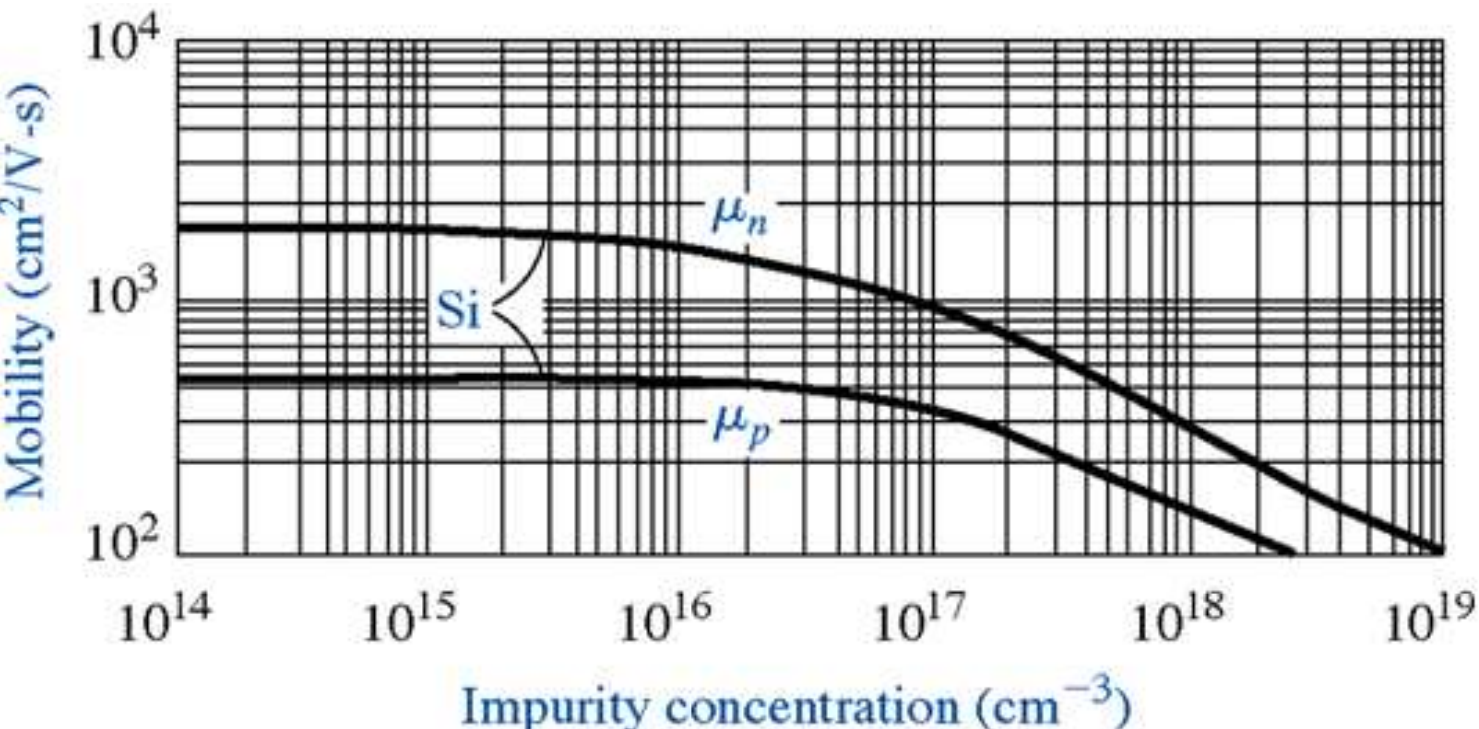
\includegraphics[width=8cm,height=4cm]{Si.png}
 \end{figure}


\section*{一、填空题}
1.由完全相同的一种原子构成的格子,格子中只有一个原子,称为\uline{\makebox[7em]{}}。满足$\vec{a_i}\cdot\vec{b_j}
=2\pi\delta_{ij}=\begin{cases}
    2\pi\quad(i=j)\\
    0\quad\quad(i\neq j)
\end{cases}$关系的$\vec{b_1},\vec{b_2},\vec{b_3}$为基矢,由$\vec{G_h}=h_1\vec{b_1}+h_2\vec{b_2}+h_3\vec{b_3}$
构成的格子,称作\uline{\makebox[4em]{}}。由若干个布拉菲格子相套而成的格子,叫做\uline{\makebox[6em]{}}。其
原胞中有\uline{\makebox[3em]{}}以上的原子。\\
2.对于固体的能带,简约波矢k的取值范围要求在\uline{\makebox[9em]{}}区域内,其取值总数等于\uline{\makebox[3em]{}}
的总数。\\
3.对于金属的能带,除填满电子的一系列能带后,还有部分被填充的能带,后者称为\uline{\makebox[3em]{}};对于半导体材料的
能带,最高填充的能带称为\uline{\makebox[3em]{}},其上最低的空带称为\uline{\makebox[3em]{}}。\\
4.如果一些能量区域中,波动方程不存在具有布洛赫函数形式的解,这些能量区域称为\uline{\makebox[3em]{}};能带的表示有
\uline{\makebox[12em]{}}、\uline{\makebox[12em]{}}、\uline{\makebox[12em]{}}三种图景。\\
5.电子在三维周期性晶格中波函数的方程的解具有\uline{\makebox[15em]{}}的形式,式中\uline{\makebox[4em]{}}在
晶格平移下保持不变(具有平移对称)。\\
6.对于4族元素Si,5族元素P作为杂质,1个P原子将可提供1个\uline{\makebox[3em]{}},属于\uline{\makebox[2em]{}}
主杂质,3族元素B作为杂质,1个B原子将提供1个\uline{\makebox[3em]{}},属于\uline{\makebox[2em]{}}主杂质。\\
7.能带顶部电子的有效质量为\uline{\makebox[2em]{}}(填写正,或负);能带底部电子的有效质量为\uline{\makebox[2em]{}}
(填写正,或负)。\\
8.温度升高,金属的导电率\uline{\makebox[3em]{}},半导体的导电率\uline{\makebox[3em]{}}。对于金属,温度越高,
金属中的晶格振动对电子的散射作用\uline{\makebox[3em]{}},而在半导体中则是有更多的电子从\uline{\makebox[3em]{}}
激发到\uline{\makebox[3em]{}}中。\\
\section*{二、简述题}
1.根据能带理论简述金属、半导体和绝缘体的导电性;并解释为什么半导体掺杂可以提高其导电能力?\\
2.简述如何利用近自由电子近似模型得到能带图。\\
\section*{三、计算题}
1.一价金属具有体心立方结构,晶格常数$a$为\AA,试求费米面的半径和费米能量。\\
2.有一补偿型非本征硅半导体,施主和受主杂质浓度均为$2.5\times10^{-17}cm^{-3}$,试计算该材料的电导率。\\

\newpage
\section*{一、填空题答案}
1.\ding{172}布拉菲格子\makebox[2em]{}
\ding{173}倒格子\makebox[2em]{}
\ding{174}复式格子\makebox[2em]{}
\ding{175}两个\\
2.\ding{172}第一布里渊区\makebox[2em]{}
\ding{173}原胞\\
3.\ding{172}导带\makebox[2em]{}
\ding{173}价带\makebox[2em]{}
\ding{174}导带\\
4.\ding{172}禁带\makebox[2em]{}
\ding{173}简约布里渊区图景\makebox[2em]{}
\ding{174}周期布里渊区图景\makebox[2em]{}
\ding{173}扩展布里渊区图景\\
5.\ding{172}$\psi_{\vec{k}}(\vec{r}+\vec{R_n})=e^{i\vec{k}\cdot\vec{R_n}}u_{\vec{k}}(\vec{r})$\makebox[2em]{}
\ding{173}$u_{\vec{k}}(\vec{r})$\\
6.\ding{172}电子\makebox[2em]{}
\ding{173}施\makebox[2em]{}
\ding{174}空穴\makebox[2em]{}
\ding{175}受\\
7.\ding{172}负\makebox[2em]{}
\ding{173}正\\
8.\ding{172}减小\makebox[2em]{}
\ding{173}增大\makebox[2em]{}
\ding{174}越大\makebox[2em]{}
\ding{175}导带\makebox[2em]{}
\ding{176}价带\\
\section*{二、简述题答案}
1.\ding{172}金属:价带完全填充,导带部分填充,导带中的电子导电。\\
\ding{173}绝缘体:价带完全填充,导带是空带,都不能导电。带隙宽,价带中的电子很难被激发到导带上。\\
\ding{174}半导体:价带完全填充,导带是空带,但是带隙较窄。室温下,价带的一部分电子可以热激发到导带上,导带和价带都变成部分
填充,可以导电。\\
\ding{175}掺杂:杂质分为施主和受主。施主能级位于带隙中接近导带的位置,其电子在室温下可以被激发到导带中;受主能级位于带隙中
接近价带的位置,价带电子在室温下可以被激发到受主能级上。因此,杂质可以改善半导体的导电性能。\\
2.使用自由电子的波函数和周期势场的平均值$\overline{V}$作为零级近似,周期势场的起伏量$Delta V=V-\overline{V}$作为微扰。
在布里渊区边界,能级是简并的,使用简并微扰处理,能级劈裂成两个,即能带之间的带隙。\\
\section*{三、计算题}
1.设近自由电子浓度为$n$,费米球半径为$k_F$,费米能量为$E_F$,则
\begin{equation*}
    \begin{aligned}
        &n=\frac{2}{a^3}=\frac{2}{(3\times10^{-10})^3}=7.4\times10^{28}m^{-3}\\
        &k_F=(3\pi n)^{\frac{1}{3}}=1.3\times10^{10}m^{-1}\\
        &E_F=\frac{\hbar^2k_F^2}{2m_0}=1.02\times10^{-18}J=6.4eV\\
    \end{aligned}
\end{equation*}
2.对于完全补偿半导体,载流子浓度为本证载流子浓度,电子和空穴浓度相同,$n=5\times10^{17}cm^{-3}$,杂志总浓度为$5\times10^{17}
cm^{-3}$。电子迁移率为$400cm^2/v\cdot s$,空穴迁移率为$190cm^2/v\cdot s$。$\mu_n=400cm^{-3}/v\cdot cm^{-1}/s$,
$\mu_p=178cm^{-3}/v\cdot cm^{-1}/s$,$n_i=1.5\times10^{10}cm^{-3}$。电导率为$\sigma=en_i(\mu_n+\mu_p)=1.4\times10^{-6}
(\Omega cm)$



\end{document}